%! Author = adnansiddiquei
%! Date = 05/03/2024

% Preamble
\documentclass[a4paper,11pt]{article}
\pdfoutput=1

% Packages
\usepackage{jcappub}
\usepackage[T1]{fontenc}
\usepackage{listings}
\usepackage{roboto}
\usepackage{subcaption}
\usepackage{blindtext}
\usepackage{seqsplit}

%\newcommand{\inlinecode}[1]{\lstinline{#1}}
%\newcommand{\inlinecode}[1]{\texttt{#1}}
\newcommand{\inlinecode}[1]{\texttt{\seqsplit{#1}}}
\lstset{basicstyle=\fontfamily{pcr}\selectfont}


\title{\boldmath M2: Applications of Machine Learning - Coursework Assignment}

% %simple case: 2 authors, same institution
\author{Adnan Siddiquei}
\affiliation{University of Cambridge}

% e-mail addresses: one for each author, in the same order as the authors
\emailAdd{as3438@cam.ac.uk}
\note{Word Count: 2412 (including figure captions and appendix).}


\begin{document}
\maketitle
\flushbottom


%! Author = adnansiddiquei
%! Date = 19/03/2024

\section{Overview of Diffusion Model Implementation}\label{sec:q1a}
\subsection{coursework\_starter.ipynb}\label{subsec:q1a}
The code provided in the coursework\_starter.ipynb notebook trains a regular denoising diffusion probabilistic model
(DDPM) on the MNIST dataset, using the \inlinecode{pytorch} library.
This section provides a detailed explanation of how the given coursework\_starter.ipynb code works.
The notation used in this section adheres to the conventions used in Ch.18 of Understanding Deep Learning, Prince~\cite{prince}.

\subsubsection{The Data}\label{subsubsec:data}
The code loads the MNIST dataset (60000 images) and preprocesses it with \inlinecode{transforms.toTensor} which converts
the image to a tensor and scales it to the range $[0, 1]$, followed by \inlinecode{transforms.Normalize((0.5,), (1.0))}
which shifts the range to $[-0.5, 0.5]$.
The scaling and range shift can help improve the training dynamics.
Given that MNIST images are grayscale (a single channel), the input dimensions are 1x28x28.
The dataset is then loaded into a \inlinecode{DataLoader} object with a batch size of 128, yielding 468 batches per
epoch.

\subsubsection{The CNN Model}\label{subsubsec:cnn-model}
The code defines a Convolutional Neural Network \inlinecode{CNN} class which is the neural network that is used to
learn the diffusion process - the noise that is added to the image at each step.
This is instantiated with 5 hidden layers, each outputting: 16, 32, 32, 16, 1 channels respectively, with a kernel size
of 7 at the first 4 layers, and a kernel size of 3 at the last layer.
Each of the first 4 hidden layers (defined in the \inlinecode{CNNBlock} class) are composed of a 2D convolutional layer
(with 0-padding on the edges) followed by a normalisation layer (\inlinecode{LayerNorm} which normalises each input to
standard normal) and a GELU activation function.
The normalisation stabilises the activations and places them in the transition range of the GELU function, which allows
for full use of the GELU's characteristics.

Decoder models for the diffusion process can either be a set of multiple models, each trained to revert the noise at
a particular step, or a single model trained to revert the noise at any given step by injecting information about the
time step into the model.
This CNN is the latter, and the \inlinecode{forward} function adds a time step dependent embedding to the pre-activations
of the second layer so that the CNN can learn to revert the noise at any given step.

\subsubsection{The DDPM Model}\label{subsubsec:ddpm-model}
\begin{figure}[t]
    \centering
    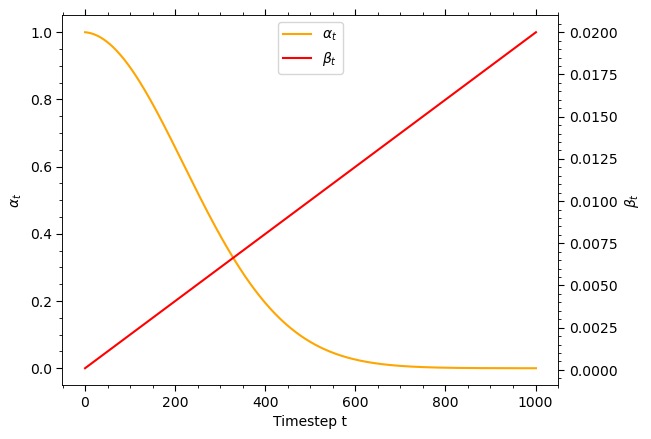
\includegraphics[width=0.8\textwidth]{figures/q1a_noise_schedule}
    \caption{A plot of $\beta_{t}$ and $\alpha_{t}$ for the linear noise schedule used in coursework\_starter.ipynb.
        This figure illustrates that MNIST images transition for noiseless to standard normally distributed noise
        over 1000 steps, with most of the noise being added by about the 600'th step.}
    \label{fig:q1a_noise_schedule}
\end{figure}

The training and sampling process is defined within the \inlinecode{DDPM} class, which contains a \inlinecode{forward}
function that defines the forward pass of the model and a
\inlinecode{sample} function that generates new MNIST data samples by iterating backwards through the diffusion process.
The DDPM is instantiated with the CNN defined above and a linear noise schedule with $\beta_{t}$ in the range $[10^{-4},
0.02]$ across 1000 steps, as shown in Figure~\eqref{fig:q1a_noise_schedule}, where $\beta_{t}$ and $\alpha_{t}$ are as
defined in Ch.18 Prince~\cite{prince}.

\begin{figure}[t]
    \centering
    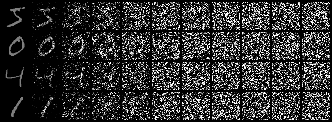
\includegraphics[width=0.8\textwidth]{figures/q1a_image_noising}
    \caption{An illustration of the linear noise schedule applied to the first 4 MNIST images in the training datastet.
        The first column shows the original 28x28 image, and the subsequent 10 columns show the image after 100 steps
        of the diffusion process.
        The final column shows the image after 1000 steps.}
    \label{fig:q1a_image_noising}
\end{figure}

The \inlinecode{forward} function samples 128 (the batch size) random $\alpha_{t}$ values from the noise schedule and
a standard normally distributed noise tensor of shape \inlinecode{(128, 1, 28, 28)}, and degrades every image in the batch
with the noise according to Equation~\eqref{eq:noise-schedule}~\cite{prince}.
\begin{equation}\label{eq:noise-schedule}
    z_{t} = \sqrt{\alpha_{t}} \cdot \mathbf{x} + \sqrt{1 - \alpha_{t}} \cdot \mathbf{\epsilon}
\end{equation}
Figure~\eqref{fig:q1a_image_noising} illustrates the diffusion process.
This batch of 128 noisy MNIST images (degraded to different extents) is then passed through the CNN (along with the
corresponding time steps) to make a prediction on the noise that was added to the image at the corresponding step.
The function returns the loss between the actual noise and this predicted noise as the mean squared error between the
two.

\begin{figure}[t]
    \centering
    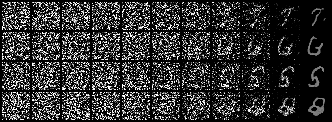
\includegraphics[width=0.8\textwidth]{figures/q1a_image_reconstruction}
    \caption{An illustration of the generation process.
        This is the generation of 4 new MNIST samples from the model trained with the default parameters in the
        coursework\_starter.ipynb notebook.
        The first column shows the randomly sampled noise, the next 10 columns illustrate the image after 100 steps of
        decoding, with the final column showing the final generated image.}
    \label{fig:q1a_image_reconstruction}
\end{figure}
The \inlinecode{sample} function can generate new MNIST samples by iterating backwards through the diffusion process
using the learned parameters of the CNN, and a random sample of standard normal noise.
Figure \eqref{fig:q1a_image_reconstruction} illustrates the generation process.

\subsubsection{The training loop}\label{subsubsec:training-loop}
The training loop iterates over 100 epochs, using the Adam optimiser and a learning rate of $2 \times 10^{-4}$,
saving generated samples from the model at every epoch along with the loss at each epoch.

%! Author = adnansiddiquei
%! Date = 19/03/2024

\section{Training the model}\label{sec:q1bc}
\begin{figure}[t]
    \centering
    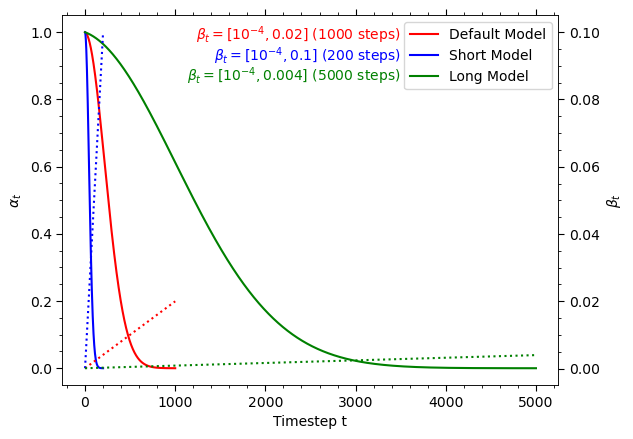
\includegraphics[width=0.8\textwidth]{figures/q1b_noise_schedules}
    \caption{A plot of each noise schedule that was evaluated.
        The dotted lines represent the $\beta_{t}$ values and the solid lines represent the $\alpha_t$ values.}
    \label{fig:q1b_noise_schedules}
\end{figure}

\begin{figure}[t]
    \centering
    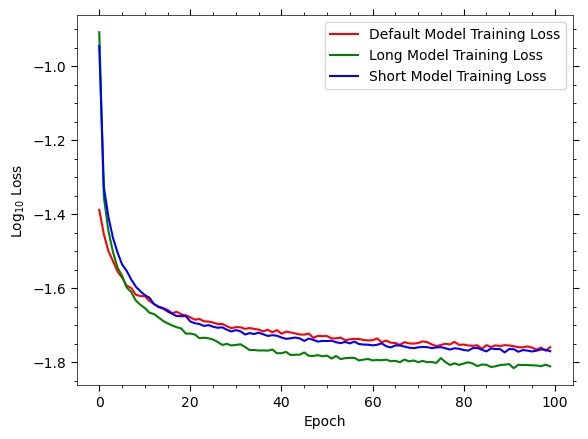
\includegraphics[width=0.8\textwidth]{figures/q1b_training_loss}
    \caption{A plot of the training loss for each model over 100 epochs.}
    \label{fig:q1b_training_loss}
\end{figure}

\begin{figure}
\centering
\begin{subfigure}{0.8\textwidth}
    \centering
    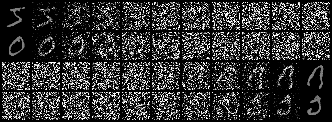
\includegraphics[width=1\textwidth]{./figures/q1b_long_model_nd}
    \caption{The noising (top 2 rows) and denoising (bottom 2 rows) process for the long model, with each column
        representing equal time steps apart (500 time steps).}
    \label{fig:q1b_long_model_nd}
\end{subfigure}%
\hfill
\begin{subfigure}{0.8\textwidth}
    \centering
    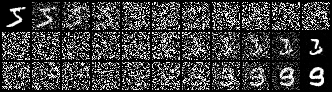
\includegraphics[width=1\textwidth]{./figures/q1b_short_model_nd}
    \caption{The noising (top 2 rows) and denoising (bottom 2 rows) process for the short model, with each column
        representing equal time steps apart (20 time steps).}
    \label{fig:q1b_short_model_nd}
\end{subfigure}
\caption{The noising and denoising process for the long and short models.
    These images illustrate the same process illustrated for the default model in Figure~\eqref{fig:q1a_image_noising}
    and Figure~\eqref{fig:q1a_image_reconstruction}.}
\label{fig:q1b_short_long_model_nd}
\end{figure}

This section discusses the training of the DDPM model with varying linear noise schedules.

Three different models were trained, the first model (default model) was trained with the provided noise schedule:
$\beta_{t} = [10^{-4}, 0.02]$ with 1000 steps; the second model (the "long model") was trained with a longer noise schedule:
$\beta_{t} = [10^{-4}, 0.004]$ with 5000 steps which added less noise at each step; and the third model (the "short model")
was trained with a shorter noise schedule: $\beta_{t} = [10^{-4}, 0.1]$ with 200 steps which added more noise at each step.
The number of steps was amended for each model such that the final noise level was the same for each model ($\alpha_{t}$
of the order of $10^{-5}$ at the final time step).
Figure~\eqref{fig:q1b_noise_schedules} illustrates the noise schedules used for each model and Figure~\eqref{fig:q1b_training_loss}
shows the training loss for each model over 100 epochs.


%! Author = adnansiddiquei
%! Date = 19/03/2024

\section{Custom Degradation - Fashion MNIST Degradation}\label{sec:q2}
A fashion MNIST degradation was implemented to train the diffusion model to generate MNIST digits.
This section discusses the design of this model, the training process and a comparison of this model with the 3 models
trained in Section~\eqref{sec:q1bc}.

\subsection{Model Design}\label{subsec:model-design}
\begin{figure}[t]
    \centering
    
\includegraphics[width=0.8\textwidth]{figures/q2_encoding}
    \caption{The encoding process for the fashion MNIST diffusion model.}
    \label{fig:q2_encoding}
\end{figure}

The exact same CNN architecture was used as in Section~\eqref{sec:q1bc} to learn the diffusion process.
The primary differences were the \inlinecode{forward} and \inlinecode{sample} functions, with the sampling process
derived from Bansal et al., (2022)~\cite{bansal}.

The forward function worked in a similar way to the \inlinecode{DDPM} models.
Degradation was applied onto the training data using Equation~\eqref{eq:schedule}, where $\epsilon$ was a randomly
sampled fashion MNIST image instead of standard normal noise.
In this way, a similar system for noise schedules could be applied, and as such, the fashion MNIST degradation was
applied using the default noise schedule of $\beta_{t} = [10^{-4}, 0.02]$ in 1000 steps.
Everything else with regard to the training process remained identical to the DDPM models detailed in Section~\eqref{sec:q1bc}.

Unconditional sampling was used for the sampling process where a random fashion MNIST digit from the test set was chosen
as the initial image and MNIST digits were generated by iterating backwards through the diffusion process.
This reverse process was implemented using Algorithm 2 from Bansal et al., (2022)~\cite{bansal}.

\subsection{Model Training and Analysis}\label{subsec:model-training}
\begin{figure}[t]
    \centering
    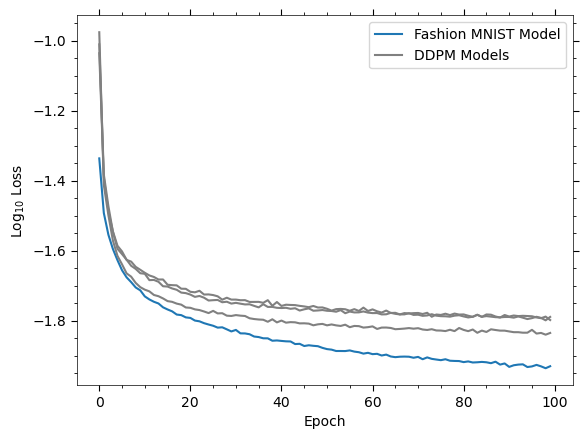
\includegraphics[width=0.8\textwidth]{figures/q2_training_loss}
    \caption{The training loss for the fashion MNIST diffusion model.
        The loss for the DDPM models from Section~\eqref{sec:q1bc} is also shown in grey for comparison.}
    \label{fig:q2_training_loss}
\end{figure}

\begin{figure}[t]
    \centering
    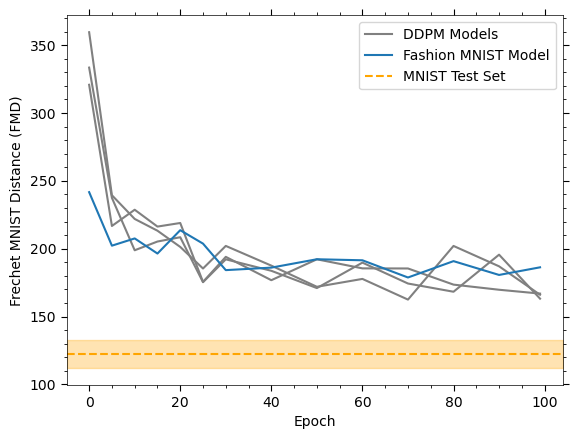
\includegraphics[width=0.8\textwidth]{figures/q2_fmd}
    \caption{The FMD values for the fashion MNIST diffusion model.
        The FMD values for the DDPM models from Section~\eqref{sec:q1bc} are also shown in grey for comparison.}
    \label{fig:q2_fmd}
\end{figure}

\begin{figure}[t]
    \centering
    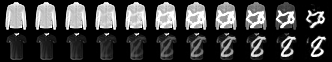
\includegraphics[width=0.8\textwidth]{figures/q2_decoding}
    \caption{The decoding process for the fashion MNIST diffusion model shown with two samples with the trained model.}
    \label{fig:q2_decoding}
\end{figure}

\begin{figure}[t]
    \centering
    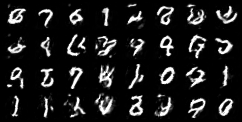
\includegraphics[width=0.8\textwidth]{figures/q2_samples_final}
    \caption{32 samples generated from the trained fashion MNIST diffusion model.}
    \label{fig:q2_samples_final}
\end{figure}

Figure~\eqref{fig:q2_samples_final} shows the training loss for the fashion MNIST diffusion model (FMDM) over 100 epochs, and
Figure~\eqref{fig:q2_fmd} shows the FMD for samples generated from the trained model at varyin epochs.
Whilst the train loss for the FMDM reached lower values than the DDPM models, the FMD values for all models were
not significantly different and inspecting the samples generated by the FMDM in Figure~\eqref{fig:q2_samples_final}
indicates no significant difference in the quality of the samples generated by the FMDM compared to the DDPM models.
It is also worth noting, whilst the FMDM had lower training loss, the loss criterion for both models were slightly
different in that the FMDM was trained to predict the input \inlinecode{x} given a degraded image, whilst the DDPM models
were trained to predict the noise added in the previous step.
Therefore, the loss curves are not as directly comparable as the FMD values are, which combined with the visual inspection,
indicate no significant difference between the two degradations.

Given that all models were allowed to train for sufficient time that the loss curve had plateaued, it is fair to conclude
that neither of these 4 models produce samples that are consistently realistic and visually similar to real MNIST
digits.
It is possible that more realistic sample could be generated with different (non-linear) noise schedules, or it is also
entirely possible that the current capacity of the CNN architecture is not sufficient to learn the diffusion process
for MNIST digits.
Further investigation would be required to assess which of these is the case, but it is likely that the latter is the
case.

%! Author = adnansiddiquei
%! Date = 19/03/2024

\section{Conclusion}\label{sec:conclusion}
In conclusion, this report has detailed the training of a diffusion model on the MNIST dataset using 3 different linear
noise schedules for a DDPM and a custom diffusion model using a fashion MNIST degradation.
All 4 models generated models that were statistically and visually similar in fidelity to each other, but relatively
poor compared to the original MNIST dataset.
It is likely that the CNN architecture used was not complex enough to capture the full complexity of the diffusion processes,
but more investigation will need to be done to confirm this.


\clearpage
\appendix

\section{MNIST Classifier Details}\label{app:mnist-classifier}
The MNIST classifier model is a CNN composed of 4 \inlinecode{CNNBlocks} ($[32, 64, 128, 64]$ channels per block) followed by an
\inlinecode{nn.AdaptiveAvgPool2d} to lower the dimensionality of the penultimate feature vector to 1024 before it is fed into
a fully connected \inlinecode{nn.Linear} layer with 10 output units (one for each class in the MNIST dataset).
This classifier was trained for 21 epochs with a batch size of 128 and a learning rate of $2 \times 10^{-4}$ using the Adam optimiser.
The loss function used was the cross-entropy loss function and the test set classification accuracy reached was 99.34\% on
the final epoch.
To extract the 1024-length feature vector, the final \inlinecode{nn.Linear} layer was set to \inlinecode{nn.Identity}
so that the model outputted the penultimate layer feature vector instead of the class predictions.
The model was trained on the MNIST training set and the test set was used for evaluation of the FMD.

\begin{thebibliography}{99}

\bibitem{prince}
Simon J.D.\ Prince,
\textit{Understanding Deep Learning}.
The MIT Press, 2023.
Available at \url{https://udlbook.github.io/udlbook/} [Accessed: 20-Mar-2024].

\bibitem{bansal}
Bansal et al.,
\textit{Cold Diffusion: Inverting Arbitrary Image Transforms Without Noise}.
University of Maryland and New York University, 2022.
Available at \url{https://arxiv.org/pdf/2208.09392.pdf} [Accessed: 28-Mar-2024].

\end{thebibliography}



\end{document}
